\documentclass{article}
\usepackage{iclr2027_conference,times}

\usepackage{hyperref}
\usepackage{url}
\usepackage{graphicx}
\usepackage{booktabs}
\usepackage{amsmath}
\usepackage{amssymb}
\usepackage{amsthm}

\graphicspath{{../../figures/}}

\newtheorem{proposition}{Proposition}
\newcommand{\rnull}{\rho_{\mathrm{null}}}
\newcommand{\rseed}{\rho_{\mathrm{seed}}}

\title{The Control Decides the Answer: \\ A Matched-Operator Null for Explanation Change
Under Model Updates}

% Authors must not appear in the submitted version. The style file prints
% "Anonymous authors / Paper under double-blind review" for as long as \iclrfinalcopy stays
% commented out, so this block is ignored during review and is filled in for the camera ready.
\author{Anonymous authors \\
Paper under double-blind review}

%\iclrfinalcopy % Uncomment for the camera-ready version, but NOT for submission.

\begin{document}
\maketitle

\begin{abstract}
When a deployed model is updated in response to a distribution shift, its feature attributions move.
Existing work measures how far they move and treats the residual, after conditioning on prediction
change, as instability. That is not yet a criterion, because it carries no account of how far an
explanation \emph{should} have moved. We supply one. Using shift families whose Bayes-optimal
predictor is available in closed form, we define a warranted-change reference $\omega$ and decompose
attribution change across an update into warranted, unwarranted and explainer-noise parts. The design
turns on a control prior work does not use: a \textbf{matched-operator null}, applying the identical
update to fresh \emph{source} data, so treatment and control differ in the distribution alone and not
in the amount of training. This changes the conclusion. Across 681 runs the null reproduces a median
82\% of the movement that follows an update. On a no-shift placebo, where
the answer is fixed by construction, it returns 1.02 on an MLP and 0.98 on gradient-boosted trees
with exact TreeSHAP, while the seed-retraining floor prior work uses implicitly returns 0.32 and
1.90 on the same data, disagreeing with itself sixfold. We state the consequence for our own results
instead of leaving it to be found: against that seed floor our headline effect is inverted (median
0.31), so the case for the matched null rests on the placebo. Applying the missing control to a
published audit, 64\% of its 45 settings produce movement smaller than refitting on a resample of the
same data. Unwarranted change is real but bounded: present across MLPs over a 630$\times$ parameter
range, trees and a small ResNet, weaker on real census covariates, absent on DistilBERT. Magnitude
indicates legitimacy only once an update completes the adaptation it implies, so it fails in the
light-update regime auditors work in.
\end{abstract}

\section{Introduction}

Post-hoc feature attributions are consumed as evidence: a practitioner reads which features a model
relied on and acts on what they read. Models do not stand still. They are fine-tuned when data
drifts, retrained on refreshed samples and redeployed. Whether the evidence survives such an update
is an open question.

The question has been asked in pieces. \citet{mougan2025} compare explanation \emph{distributions}
across domains for a frozen model. \citet{fass2026} filter to prediction-preserved pairs before
measuring attribution stability under input perturbation. \citet{deltaaudit2025} difference
attributions across a model update. \citet{rsp2026} tracks attribution change across fine-tuning
epochs. Each measures a magnitude. None supplies the prior quantity, which is how far the
explanation should have moved. Absent that quantity, every method treats change as damage and names
the residual by fiat, calling it instability, semantic drift or risky reliance redistribution.

Treating all change as damage misclassifies a case that occurs in practice. A model fine-tuned on
data from which a spurious shortcut has been removed should stop attributing to that shortcut. Its
predictions on most inputs are unchanged, its explanation changes a great deal, and the change is
the desired behaviour. A metric that scores this as instability is measuring something other than
what it claims.

Two checkpoints that agree on the shared support but differ in their gradients are different
functions that the data did not distinguish, which is the underspecification phenomenon
\citep{damour2020} read through attributions. There is a second gap, and it proves to be the larger
one. Measuring how far attributions moved after
an update requires knowing how far they would have moved anyway. Prior work's implicit control is an
independent retrain with a different seed. That control differs from the treatment in operator, data
volume and step count at once, so a comparison against it does not isolate the distribution. We
supply a control that differs in the distribution alone, and find that the choice reverses the
ordering of update regimes.

\paragraph{Contributions.}
\begin{enumerate}\itemsep2pt
\item \textbf{A warranted-change reference.} We define $\omega$ as the change in the attributions of
the \emph{Bayes-optimal predictor} of each environment, not of the causal generating
mechanism. On generators where that predictor is available in closed form, $\omega$ is exact:
identically zero under covariate shift, non-zero and computable under concept shift and shortcut
removal. The definitional choice is what makes the shortcut case come out right (\S\ref{sec:warranted}).
\item \textbf{A matched-operator null.} The control for a fine-tune-on-target treatment is the
identical fine-tune on fresh \emph{source} data, matched in learning rate, epochs, step count and
sample size (\S\ref{sec:controls}, \S\ref{sec:inversion}).
\item \textbf{A decomposition, not a metric.} Every distance we use already exists
\citep{alvarez2018,yeh2019,bhatt2020,agarwal2022ros,openxai2022,quantus2023}; the contribution is
the reference and the controls.
\item \textbf{Three propositions} on which explainer classes inherit stability from prediction
stability, each with a sharpness construction and a per-point numerical check (\S\ref{sec:theory}).
\item \textbf{An empirical finding that survives its own controls}, together with an explicit account
of where it stops holding (\S\ref{sec:results}).
\end{enumerate}

\paragraph{What we do not claim.} We do not propose a new stability metric. We do not detect
distribution shift; that is the contribution of \citet{mougan2025}, whose frozen-model setting is not
ours. We were not first to condition on prediction preservation; \citet{fass2026} were, and we adopt
their conditioning. We avoid the phrase ``explanation drift'', which denotes at least three distinct
objects in the 2025--2026 literature (Appendix~\ref{app:terms}).

\section{Setup and related work}

\paragraph{A category error worth stating once.} For a frozen model $f$ and a deterministic explainer
$E$, the explanation $E_f(x)$ is a fixed function of $x$. Changing $P(X)$ does not change $E_f(x)$ at
any $x$; it changes only which $x$ are observed. Instance-level explanation change under pure data
shift with a frozen model is identically zero, and the only measurable object is the shift of the
explanation \emph{distribution}, which is what \citet{mougan2025} measure. Genuine instance-level
change requires one of: the model changed, the input changed, or the explainer is stochastic. This
paper studies the first. The second belongs to \citet{fass2026} and the adversarial-fragility line
\citep{ghorbani2019,dombrowski2019,slack2020}. The third is a nuisance we measure and subtract. We verify all
three empirically instead of asserting them (\S\ref{sec:controls-behave}).

\paragraph{Objects.} $f:\mathcal{X}\to\mathbb{R}$ is the explained scalar output, always the logit,
so that the theory, the explainers and the closed-form reference share a space. An update operator
produces $f_{t+1}=\mathcal{U}(f_t,\mathcal{D})$. A probe set $\mathcal{P}$ is drawn from the
\emph{shared support} of source and target, so neither checkpoint extrapolates on it, and the
prediction-preserved subset is
$\mathcal{P}_\epsilon=\{x\in\mathcal{P}:|p_t(x)-p_{t+1}(x)|\le\epsilon\}$. Conditioning on
preservation is not optional: Shapley efficiency implies that if two inputs' predictions differ their
attribution vectors must differ in at least one coordinate, so measuring change without conditioning
partly measures an algebraic necessity. Shifts are \emph{generated}, never assumed. Covariate shift
moves $P(X)$ with $P(Y\mid X)$ fixed, concept shift moves $P(Y\mid X)$, and shortcut removal severs a
feature that was predictive but never causal.

\begin{table}[t]
\caption{Related work organised by what changes. The last row is closest to this paper.}
\label{tab:related}
\centering\small
\begin{tabular}{@{}lll@{}}
\toprule
\textbf{What changes} & \textbf{Work} & \textbf{What is missing} \\
\midrule
data, model frozen & \citet{mougan2025} & instance-level change is vacuous here \\
the input & \citet{fass2026,ghorbani2019} & single model; residual named by fiat \\
the seed & \citet{evoxplain2025,laberge2023} & no shift; this is our \emph{floor} \\
the model class & \citet{hypclass2026} & architecture varies, distribution does not \\
the checkpoint & \citet{deltaaudit2025,rsp2026,xray2026} & no reference, no matched control \\
\bottomrule
\end{tabular}
\end{table}

A separate line explains the shift itself instead of the model's response to it
\citep{kulinski2023,hinder2022}, and a further line documents that explainers disagree with one
another on a fixed model \citep{krishna2022}. Neither supplies a reference for how far an
explanation should move. We exclude attention weights, whose status as explanation is contested
\citep{jain2019}. Table~\ref{tab:related} organises the field by the object that changes. The two nearest works deserve
specifics. \citet{deltaaudit2025} difference occlusion attributions across model pairs and label
movement uncorrelated with behaviour change ``spurious'', which is a heuristic and not a
reference, and which misfires on the shortcut case. \citet{fass2026} establish that without
conditioning on prediction preservation up to 99\% of compared pairs have changed predictions, then
measure raw distance on what remains, with no floor for comparison.

\section{Warranted change and the two controls}
\label{sec:warranted}

\paragraph{The reference.} We define $\omega$ against the Bayes-optimal predictor
$h_e(x)=\operatorname{logit}P_e(Y{=}1\mid X{=}x)$ of each environment:
\begin{equation}
\omega(x)=d\big(\phi(\mathrm{IG}[h_S](x,b)),\ \phi(\mathrm{IG}[h_T](x,b))\big).
\end{equation}
Referencing the \emph{causal} mechanism instead would invert the shortcut verdict. Under shortcut
removal the causal function is unchanged, yet a correct model must stop using the shortcut, so a
causal reference would label that change unwarranted. The Bayes reference is exactly zero under
covariate shift and available in closed form under concept shift and shortcut removal.

\paragraph{The floors.}
\label{sec:controls}
$\nu$ is the explainer's own noise, measured between two runs on one checkpoint. $\rnull$ is the
matched-operator null: the identical update applied to fresh source data, holding learning rate,
epochs, step count and sample size fixed, so that only the sampling distribution differs. $\rseed$ is
the independent-retrain floor that prior work uses. We report
\begin{equation}
\mathrm{UEC}=\textstyle\mathbb{E}_{\mathcal{P}_\epsilon}[\Delta]-\omega-\max(\nu,\rnull),
\qquad \text{ratio}=\mathbb{E}[\Delta]/\rnull .
\end{equation}
UEC is a difference and not a ratio to output change, because such a ratio
\citep{agarwal2022ros} is undefined and explosive in the prediction-preserving regime this paper
concerns. The null and the treatment contain the same optimisation transient, and only the treatment
additionally contains the distribution signal. Comparing a fine-tune against a from-scratch retrain,
as the seed floor does, confounds the operator with the distribution.

\section{Theory}
\label{sec:theory}

Let $\delta=f_t-f_{t+1}$, baseline $b$, path $\gamma(\alpha)=b+\alpha(x-b)$. All explainers below are
linear in the explained function.

\begin{proposition}[Path-integrated: the aggregate is inherited, the allocation is not]
(i) $\sum_j \Delta \mathrm{IG}_j(x)=\delta(x)-\delta(b)$ exactly, hence
$|\sum_j \Delta\mathrm{IG}_j(x)|\le 2\epsilon$ when the checkpoints agree to $\epsilon$ at $x$ and at
$b$, requiring agreement at the two endpoints only and not along the path.
(ii) $\|\Delta\mathrm{IG}(x)\|_1 \le \|x-b\|_1\sup_\gamma\|\nabla\delta\|_\infty$.
(iii) \emph{Sharpness:} output preservation alone does not bound individual components. With
$\delta(z)=\epsilon\sin(\omega(z_1-z_2))$, $b=0$, $x=\mathbf{1}$, we have $|\delta|\le\epsilon$
everywhere, yet $\Delta\mathrm{IG}_1=\epsilon\omega$ is unbounded while the aggregate is zero.
\end{proposition}

\begin{proposition}[Local gradients inherit nothing, not even the aggregate]
With $\delta(z)=\epsilon\sin(\omega z_1)$, the aggregate gap
$\sum_j \Delta(\mathrm{G}{\times}\mathrm{I})_j(x)=x_1\epsilon\omega$ is unbounded under the premise
that pins IG's aggregate to $2\epsilon$.
\end{proposition}

\begin{proposition}[Shapley, under a coalition-level premise]
If $|v_f(S)-v_{f'}(S)|\le\epsilon_{\mathrm{coal}}$ for every coalition $S$, then
$\|\varphi^f-\varphi^{f'}\|_\infty\le 2\epsilon_{\mathrm{coal}}$.
\end{proposition}

\noindent\emph{Remark.} $\epsilon_{\mathrm{coal}}$ is a supremum over masked, off-manifold inputs.
Fine-tuning optimises a loss over the data distribution and leaves the model unconstrained there, so
preservation on the data implies nothing about $\epsilon_{\mathrm{coal}}$. We measure the gap rather
than assume it (\S\ref{sec:theory-check}).

\paragraph{Corollary.} Under a prediction-preserving update, IG's aggregate attribution mass is
bounded, gradient$\times$input's is not, and Shapley's is bounded only if the coalition premise
holds. Collinearity constrains the allocation further, since attribution mass can move between
near-duplicate features without changing the function; our redundant-feature block is built to
exercise that case. No class is protected in its \emph{allocation} across features, which is the part a
practitioner reads. The sharpness construction is not exotic in kind: it is a difference that
oscillates transverse to the integration path while vanishing on it, which is to say two checkpoints
that agree on the data manifold and curve differently off it. This is the mechanism
\citet{dombrowski2019} identified in input space, transposed to model space.

\section{Experimental protocol}

Shifts are generated from a structural equation model with $d{=}20$ features in causal, shortcut,
redundant and noise blocks, for which the Bayes-optimal logit and its integrated gradients have
closed forms. Attributions target the logit; the attribution baseline is fixed across checkpoints,
since a per-checkpoint baseline makes $\Delta\mathrm{IG}$ uninterpretable. Activations are smooth by
default, because on a ReLU network IG completeness holds only to $O(1/n_{\text{steps}})$ and would
contaminate the Proposition~1 check. Gradient-boosted trees use XGBoost with exact TreeSHAP \citep{chen2016xgboost}. We use seven
explainers spanning path-integrated, local-gradient and Shapley-type classes \citep{sundararajan2017,erion2021,simonyan2013,smilkov2017,lundberg2017,
ribeiro2016,lundberg2020tree}, implemented through Captum \citep{kokhlikyan2020captum}. Beyond the
generator we use ACS Income \citep{ding2021folktables}, CIFAR-10 with common corruptions
\citep{krizhevsky2009cifar,hendrycks2019benchmarking}, and DistilBERT on IMDB
\citep{sanh2019distilbert,maas2011imdb}. Tests are paired across seeds with Holm correction
\citep{holm1979} and Cliff's $\delta$ \citep{cliff1993}. Our reading of what an attribution
evaluation must control for follows recent critiques of the evaluation protocols themselves
\citep{rethinkrobust2025}. Figures are drawn to be legible under the common colour-vision
deficiencies and in monochrome (Appendix~\ref{app:figures}).

\section{Results}
\label{sec:results}

\subsection{The controls behave, and the placebo is decisive}
\label{sec:controls-behave}

\begin{figure}[t]
\centering
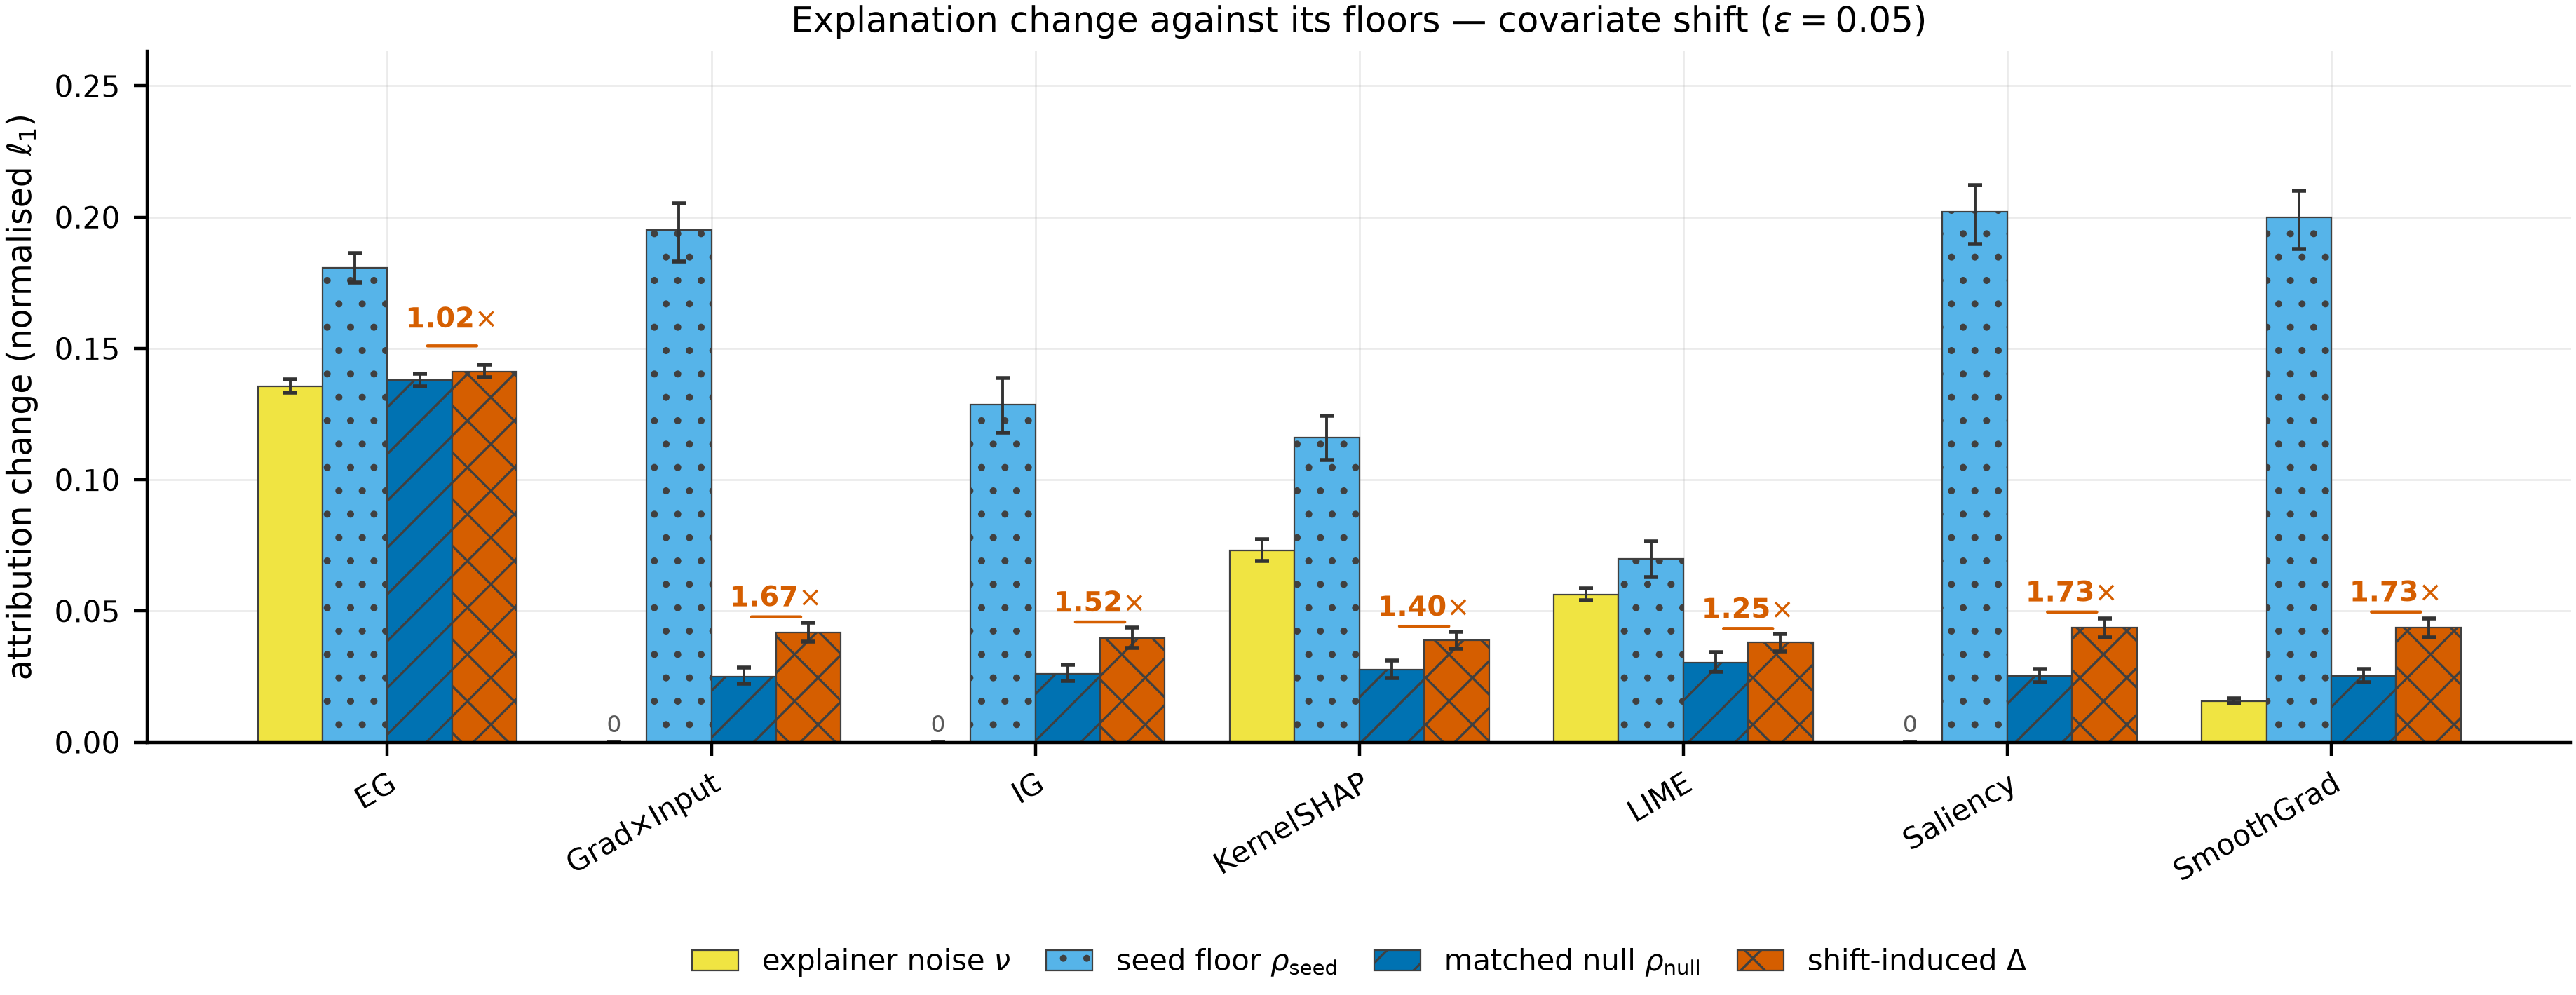
\includegraphics[width=\textwidth]{fig2_headline.png}
\caption{Attribution change against its floors under covariate shift, where $\omega$ is exactly zero,
so any movement above the matched null is unwarranted. Bars are means over seeds with bootstrap
intervals; brackets give $\Delta/\rnull$. Deterministic explainers have $\nu=0$ exactly, marked
``0''. The seed floor $\rseed$ exceeds the measured change for every explainer, which is the
observation \S\ref{sec:inversion} turns on.}
\label{fig:headline}
\end{figure}

Deterministic explainers reproduce bitwise on a fixed checkpoint, so $\nu=0$ exactly; a frozen model
under pure data shift yields identically zero instance-level change, confirming \S2 numerically
and not by assertion. On a no-shift placebo, where the correct answer is fixed in advance, the
matched null returns 1.02 on an MLP and 0.98 on gradient-boosted trees with exact TreeSHAP. The seed
floor returns 0.32 and 1.90 on the same data. It disagrees with itself sixfold across two model
classes and errs in opposite directions, so no fixed correction recovers it. This test does not
depend on any shift result and was specified before them.

\subsection{Which control you choose reverses the conclusion}
\label{sec:inversion}

\begin{figure}[t]
\centering
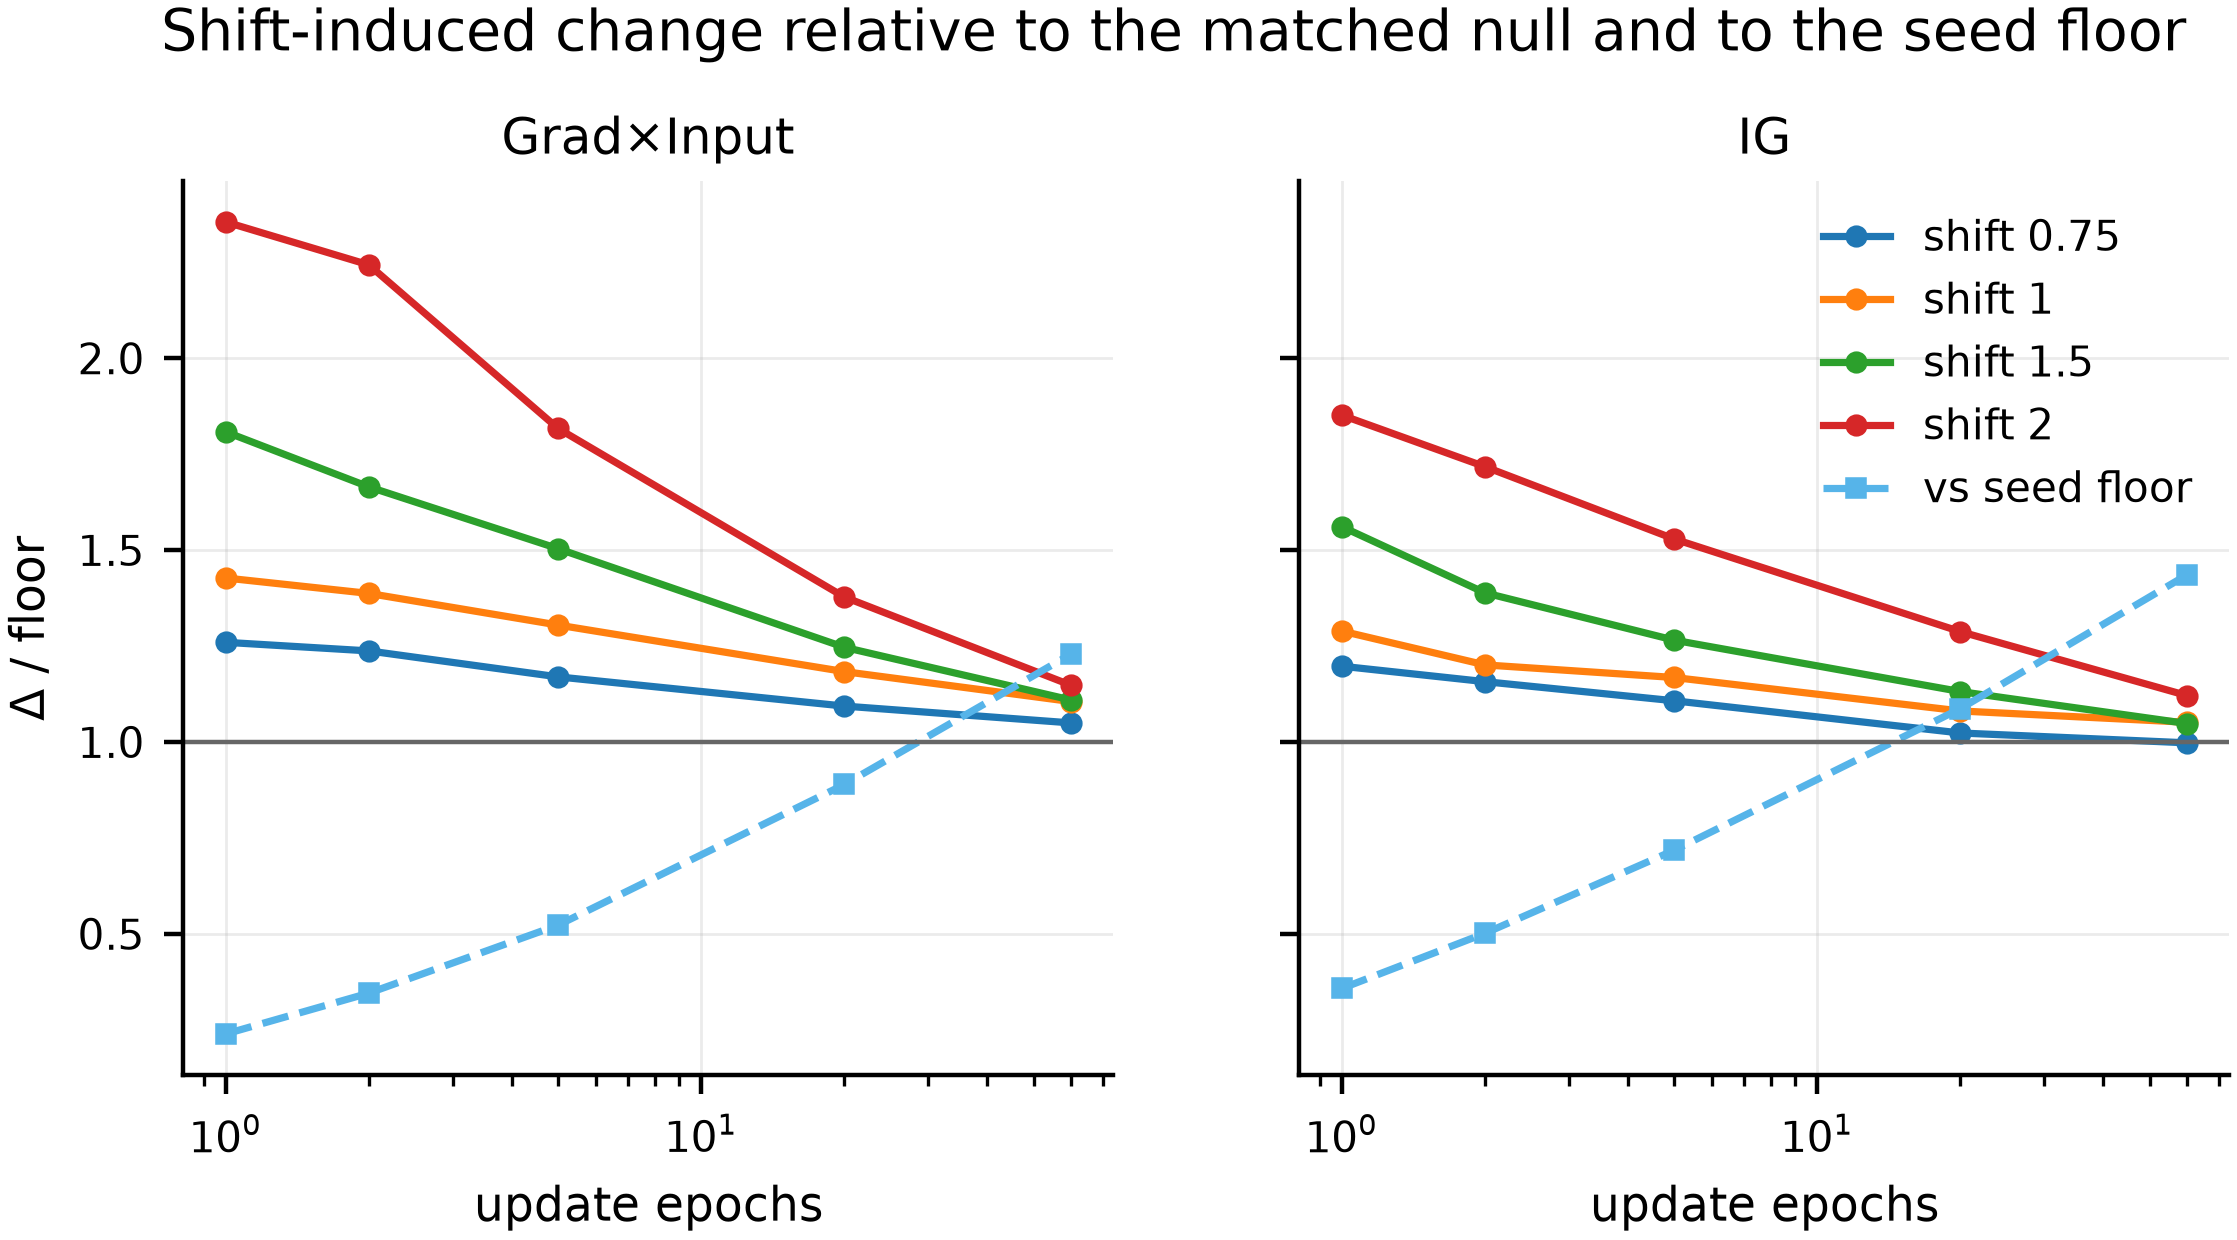
\includegraphics[width=\textwidth]{fig2b_update_strength.png}
\caption{Change relative to the matched null (solid) and to the seed floor (dashed) as the update
grows heavier. The two controls order the update regimes in opposite directions and the curves cross.
Learning rates are pooled here; the single cell quoted in the text is more pronounced.}
\label{fig:inversion}
\end{figure}

Over a grid of shift magnitude $\times$ update strength (600 runs, 5 seeds), change relative to the
matched null \emph{falls} as the update gets heavier, while change relative to the seed floor
\emph{rises} (Figure~\ref{fig:inversion}). For IG at shift magnitude 1.5 and update learning rate $2\times10^{-4}$,
$\Delta/\rnull$ runs 1.81, 1.58, 1.39, 1.28, 1.09 across 1, 2, 5, 20 and 60 epochs, while
$\Delta/\rseed$ runs 0.11, 0.19, 0.41, 0.82, 1.07. That is the most pronounced of the twelve cells,
so we report what happens in the rest: the opposite ordering holds in 24 of 24
explainer\,$\times$\,magnitude\,$\times$\,learning-rate cells, and the curves cross in 10 of 12. The
direction, which is what the argument needs, is unanimous. Read against the seed floor a heavy update
looks maximally shift-driven; read against the matched null it is the least shift-driven condition.
The reason is mechanical: the seed floor is a fixed quantity while $\Delta$ grows with training, so
the ratio to it measures how hard one trained, not how far the data moved. Across 681 runs the
matched null reproduces a median 82\% of the movement that follows an update.

\paragraph{Stated plainly: against the seed floor our headline effect is inverted.} In the
covariate-shift condition of \S\ref{sec:h1}, $\Delta/\rseed$ runs 0.21 to 0.78 with a median of 0.31.
A reader who takes seed retraining as the reference will conclude there is no phenomenon here. We put
the number in the main text because it is the first thing a sceptical reader computes, and because
our answer to it is the paper's argument and not a qualification of it. The obvious suspicion is
that we adopted whichever control produced the answer we wanted. The placebo of
\S\ref{sec:controls-behave} speaks against that, and it is decisive because its ground truth is fixed
in advance: a control that manufactures a two-fold effect from an unshifted placebo cannot certify
effects under shift. Two further points support it. The comparison is not like-for-like, since
$\rseed$ retrains from scratch on 8{,}000 points for 60 epochs while the update is 20 epochs on
4{,}000, so $\Delta/\rseed$ varies operator, data volume and step count at once. And the two controls
disagree about direction, not only magnitude; a valid-but-conservative reference would preserve the
ordering and change only the scale.

\subsection{Unwarranted change exists}
\label{sec:h1}

Under covariate shift, where $\omega$ is exactly zero, all seven explainers move more than their
matched null (Figure~\ref{fig:headline}). The ratios are 1.73 (saliency and SmoothGrad), 1.67
(gradient$\times$input), 1.52 (IG), 1.40 (KernelSHAP), 1.25 (LIME) and 1.02 (expected gradients),
with Holm-adjusted $p=0.014$ and Cliff's $\delta$ up to $+0.98$. The effect is largest for
gradient-boosted trees with exact TreeSHAP (2.08), so it is not a gradient artefact, and it persists
on a small CIFAR ResNet. It also replicates on ACS Income, where 27 of 28 explainer\,$\times$\,state
cells remain significant after Holm correction. Ablating the distance, normaliser, $\epsilon$
threshold, IG baseline, SHAP background and probe sampling leaves the ordering of conclusions
unchanged (Kendall $\tau=1.00$ across the core axes).

\subsection{Magnitude and legitimacy: a conditional result}
\label{sec:h2}

\begin{figure}[t]
\centering
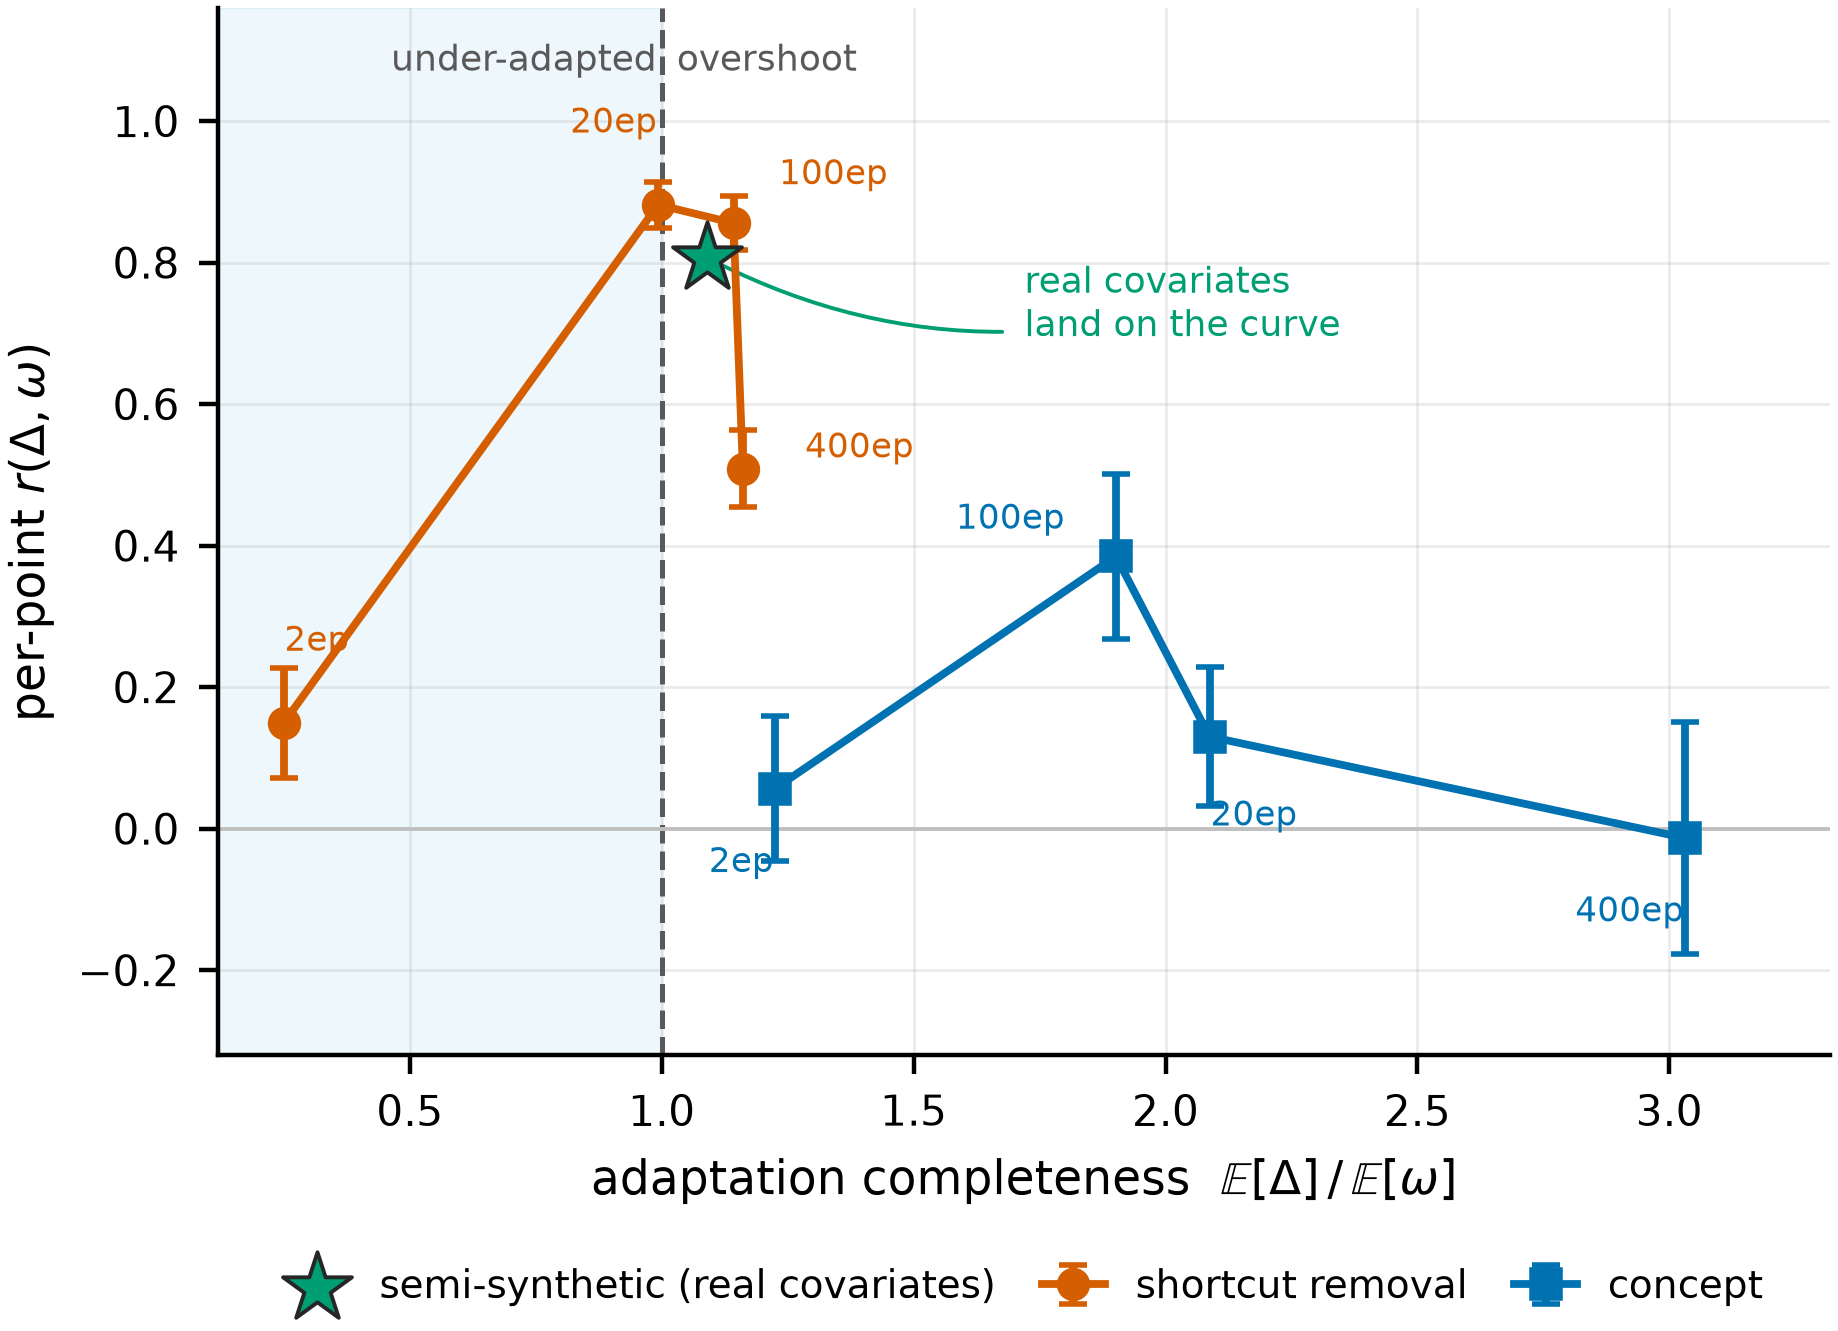
\includegraphics[width=\textwidth]{fig13_adaptation.png}
\caption{Per-point tracking of the warranted reference against how far the update actually
travelled. Sweeping the update budget carries $r$ from $+0.15$ to $+0.88$ as completeness passes
through 1, then down again on overshoot. The semi-synthetic run on real covariates lands on the same
curve, so the disagreement in \S\ref{sec:h2} is not a property of the data.}
\label{fig:adaptation}
\end{figure}

We now test whether the amount an explanation moves indicates whether it should have moved.
Within a shift family each probe point carries its own $\omega$, so measured change can be regressed
on it directly.
Correlations are computed within seed and aggregated across seeds. Under light updates the
association is small: $r=+0.121$ $[+0.084,+0.157]$ under concept shift over 3{,}237 points and
$r=-0.104$ $[-0.192,-0.015]$ under shortcut removal over 4{,}329 points, so the warranted change
accounts for roughly 1\% of the variance in the measured change. Both intervals exclude zero, so we
do not claim the association is absent, only that it is small. We report this as a magnitude with an
interval instead of testing against an equivalence margin, since any margin chosen after seeing
these numbers would be the post-hoc move this paper criticises elsewhere.

The per-explainer version of the same comparison is underpowered at ten seeds. A two one-sided test
\citep{schuirmann1987} against a $\pm 0.10$ margin, fixed from the placebo's own spread, declares
only one of seven explainers equivalent, and that one is expected gradients, whose two ratios are both
near 1.02 and whose pass therefore reports its insensitivity. LIME is a genuine exception: its ratio
is 0.64 higher under shortcut removal than under covariate shift ($p=0.002$). We name it instead of
averaging it away, while noting that its own noise floor exceeds its matched null, so we cannot
separate sensitivity from sampling variance.

\paragraph{The condition.} Repeating the measurement on real ACS covariates with a mechanism known by
construction gives $r=+0.81$, the opposite conclusion. The cause is not the covariates. Define
completeness as $\mathbb{E}[\Delta]/\mathbb{E}[\omega]$, the fraction of the warranted distance the
update actually covered; it is 0.12 and 0.54 in the two synthetic settings and 1.09 in the
semi-synthetic one. Sweeping the update budget on the generator confirms the reading
(Figure~\ref{fig:adaptation}): on shortcut removal, $r$ rises from $+0.149$ at completeness 0.249 to
$+0.882$ at completeness 0.993, then falls to $+0.509$ once the update overshoots. Distance from
perfect adaptation predicts tracking at $\mathrm{corr}(|\log\text{completeness}|,r)=-0.870$, and on
the rising limb completeness and $r$ correlate at $+0.756$. The relationship is peaked and not
monotone, which is why a naive pooled correlation of $-0.356$ would mislead. The claim is therefore
conditional: attribution magnitude tracks warranted change when the update completes the adaptation,
and under the light, prediction-preserving updates that deployment uses it carries little such
information. That is the regime auditors work in, because heavy updates which complete the adaptation
also move predictions visibly.

Two published metrics inherit the consequence. Reimplemented on the same checkpoints, a FASS-style
filtered distance and Delta-Audit's spurious residual rank correct adaptation as 45\% and 89\%
\emph{worse} than unwarranted drift, and UEC assigns them opposite signs.

\subsection{Re-auditing a published result}

Applying the missing control to \citet{deltaaudit2025}, we re-run its 45 reported settings with a
matched null. 64\% produce attribution movement smaller than refitting the same model on a resample
of the same data, and only 33\% clear that floor, with a median ratio of 0.861. Their own flagship
examples survive comfortably, which is worth stating: the conclusion is about the reported settings
in aggregate and not about the paper's headline claims.

\subsection{The theory holds, and the change is not faithfulness loss}
\label{sec:theory-check}

\begin{figure}[t]
\centering
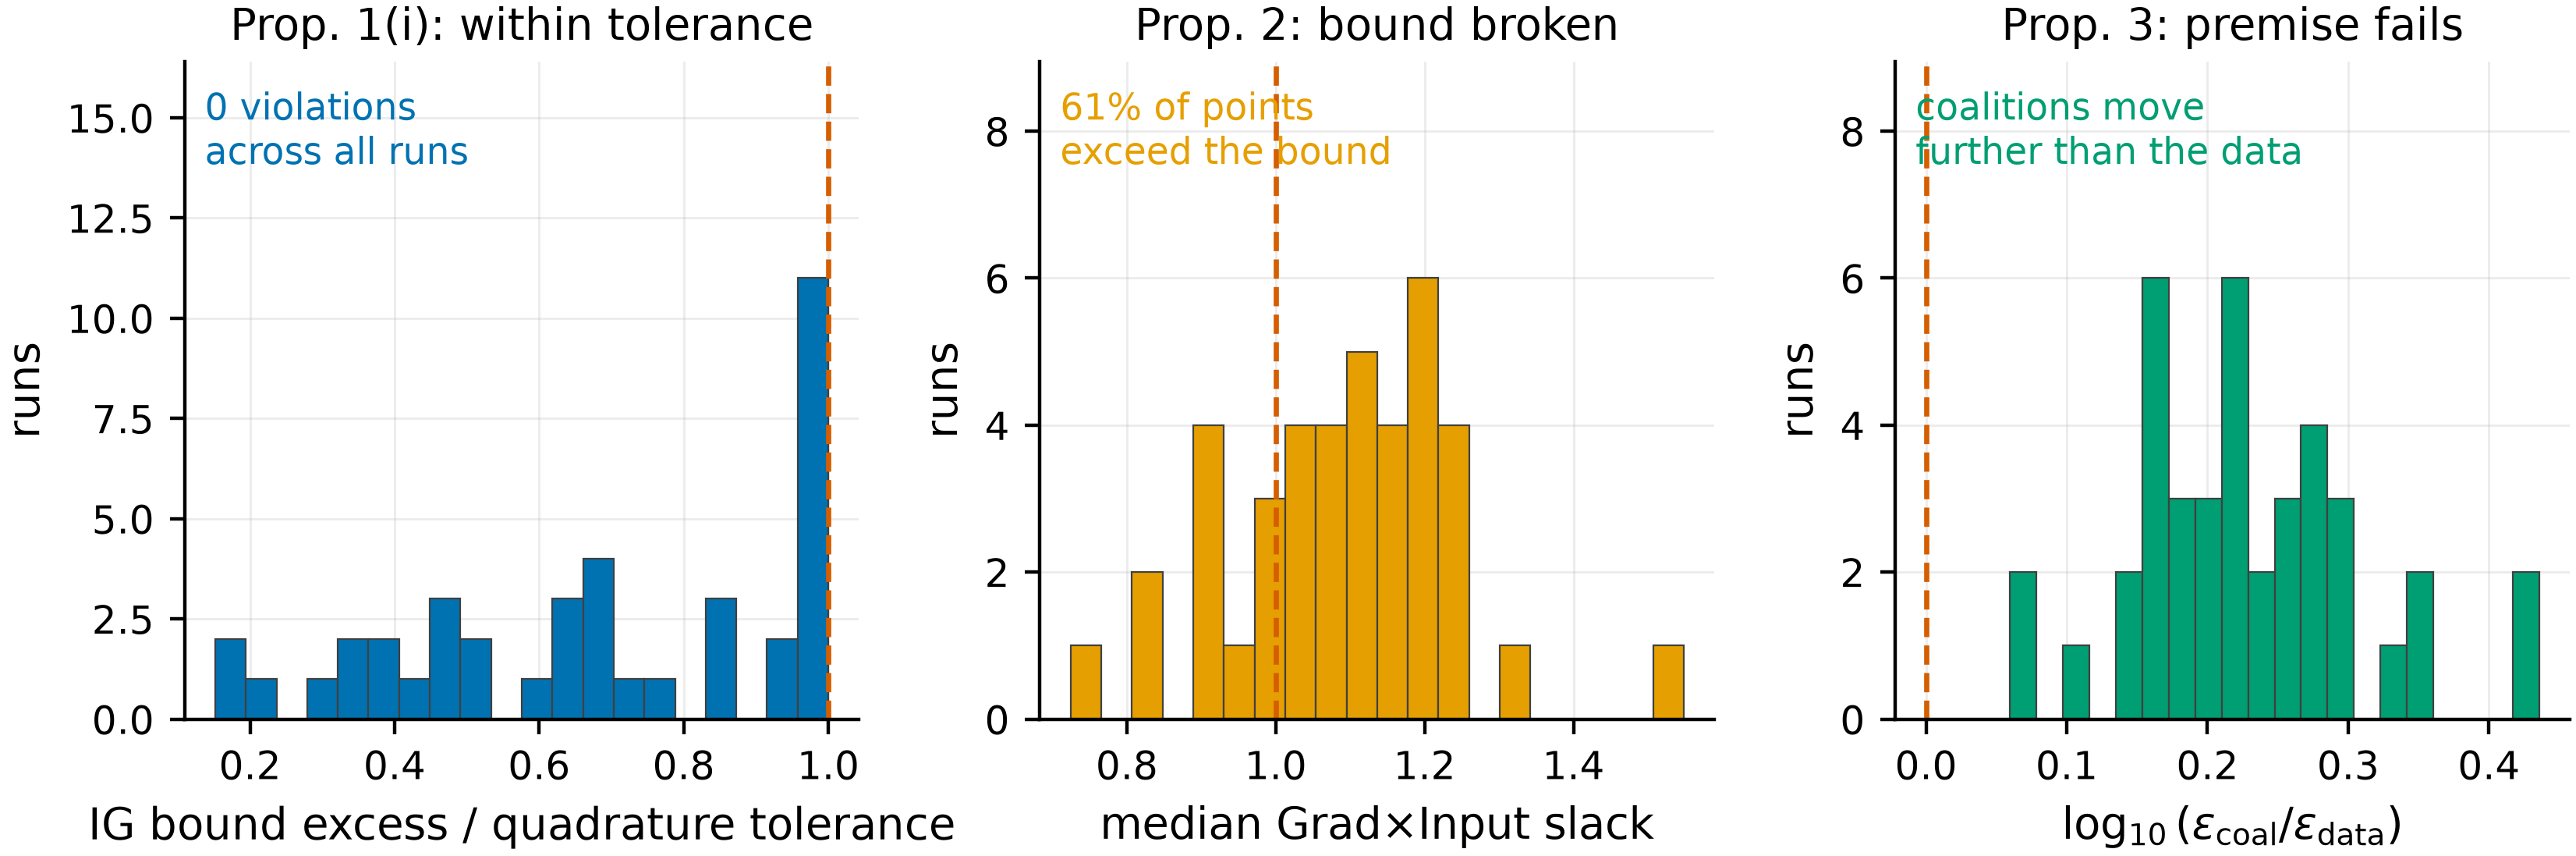
\includegraphics[width=\textwidth]{fig5_theory.png}
\caption{Per-run checks of the three propositions. Left: IG's aggregate excess over the bound,
divided by each run's own quadrature tolerance, so values below 1 are numerical. Middle:
gradient$\times$input breaks the same bound. Right: the coalition premise of Proposition~3 fails
off-manifold.}
\label{fig:theory}
\end{figure}

Proposition~1(i) records 0 violations in 20{,}000 probe points, once each run is compared against its
own quadrature tolerance (Figure~\ref{fig:theory}). Gradient$\times$input breaks the same bound on
60.8\% of points. The coalition premise of Proposition~3 fails off-manifold, with masked inputs
moving 1.49 to 2.02 times further than data inputs across shift families. Separately, the effect is
not explainers becoming wrong instead of merely different: restricting to points where the explainer
is faithful to both checkpoints leaves the ratio unchanged (1.567 against 1.563), and the correlation
between $\Delta$ and the faithfulness drop lies in $[-0.084,+0.032]$ across seed-averaged cells.

\subsection{Where the effect stops}

The effect is bounded, and we map the boundary and not the interior. It is flat at roughly 1.4
across a 630$\times$ parameter range within models trained from scratch, moving from 1.48 at 1.7k
parameters to 1.36 at 1.07M. On real census covariates with a mechanism known by construction it
weakens to 1.20 $[1.05,1.34]$ for IG, and the machinery of $\omega$ transfers exactly there, matching
quadrature to $1.1\times10^{-14}$ on real rows under a tilt calibrated to the synthetic shift's own
domain-classifier AUC (0.906 against 0.902). On DistilBERT at 66.9M parameters it is absent: 1.02
$[0.97,1.09]$, unchanged across a tenfold range of update strength.

Modelling the optimiser share directly shows that the last result is not simple extrapolation
(Figure~\ref{fig:share}, Appendix~\ref{app:share}). Capacity does not predict the share at all, with a logit-scale slope of
$-0.007$ $[-0.197,+0.184]$, $p=0.94$, across 630$\times$ of parameters. Update strength does predict
it, monotonically. At matched update size DistilBERT sits $+0.173$ $[+0.104,+0.243]$ \emph{above} the
from-scratch curve (Welch $p=3.3\times10^{-4}$). Whether that excess comes from pretraining or from
architecture, this design cannot separate.

Finally, the monitored quantity that does correlate with unwarranted change points the wrong way:
higher prediction agreement between checkpoints goes with \emph{more} unwarranted change, not less,
and target accuracy's association reverses sign across shift magnitudes.

\section{Limitations}

\textbf{The reference needs a known Bayes predictor.} $\omega$ is exact only where the generative
process is known. On real data we claim the covariate-shift null alone, and even there it is checked
through a calibration-transfer test and is not proved. The semi-synthetic construction removes the
covariate half of that assumption but not the label half, which no method can remove.

\textbf{H2 is conditional on the update completing the adaptation.} We identify the governing
quantity (\S\ref{sec:h2}) but characterise it on two shift families in one generator plus one
semi-synthetic setting. Whether completeness governs tracking elsewhere is untested.

\textbf{Scale.} DistilBERT is covered, but nothing here speaks to vision transformers, and the
$+0.173$ excess cannot be attributed to pretraining over architecture without a same-size
transformer trained from scratch.

\textbf{Our effect is smaller than the literature we critique.} Against the seed floor it is
inverted, and the case for the matched null rests on a placebo rather than on the shift results the
control is used to interpret. A reader who rejects the placebo argument should reject the paper's
empirical claims with it.

\section{Conclusion}

The measurement of explanation change after a model update turns on a control that has not been
used. Applying the identical update to fresh source data isolates the distribution from the
optimisation, and it reverses the ordering that a seed-retraining floor produces. Most of the
attribution movement reported after fine-tuning is reproduced by the optimiser alone. A reference for
how far explanations should have moved makes the remaining question askable, and answers it
conditionally: magnitude indicates legitimacy when an update completes the adaptation it implies, and
carries little information under the light updates that deployment uses.

\subsubsection*{Ethics statement}

This work uses only public datasets and involves no human subjects, no personally identifying
information and no new data collection. ACS Income \citep{ding2021folktables} is derived from public
census microdata and carries demographic attributes including sex and race, which our models consume
as features because the published prediction task does. We make no fairness claim and use the data
solely to test whether a measurement design transfers from a generator to real covariates; the
attribution changes we report should not be read as evidence about any group. The paper is
diagnostic in aim, and the plausible misuse we can foresee is that a practitioner reads unwarranted
attribution change as a fairness finding, which \S\ref{sec:h2} argues directly against. The authors
have read the ICLR Code of Ethics and adhere to it.

\subsubsection*{Reproducibility statement}

Every quantitative claim is regenerated from the released code. A single entry point runs all
fourteen stages in dependency order and rebuilds every table and figure. A verification script
re-derives 80 headline numbers from the produced artefacts and fails if any drifts, and 101 tests
cover the generator, the operators and a numerical check of each proposition. Figures write their
source data beside the image. The synthetic and semi-synthetic pipelines run on CPU; the transformer
arm requires one GPU and its measured output is committed so the rest reproduces without it. Code is
supplied as anonymised supplementary material.

\subsubsection*{Use of AI statement}

Large language models were used as a coding and editing assistant: drafting and refactoring
experiment code, proposing figure layouts, and copy-editing prose. All experimental design decisions,
the choice of reference and controls, the propositions and their proofs, and every claim in this
paper were made and checked by the authors. Every number reported here is produced by the released
code and re-derived by the verification script described above.


\bibliographystyle{iclr2027_conference}
\bibliography{references}

\appendix

\section{Terminology: what ``explanation drift'' denotes}
\label{app:terms}

The phrase names at least three distinct objects in the 2025--2026 literature, which is why we avoid
it. \citet{mougan2025} use \emph{explanation shift} for a divergence between $P(E_f(X_S))$ and
$P(E_f(X_T))$ for a frozen model, a population-level object. \citet{rsp2026} uses \emph{explanation
drift} for the epoch-to-epoch change of attributions on a fixed probe set within a single training
run. The concept-drift literature uses \emph{drift explanation} for the opposite direction of
inference, explaining why the data moved \citep{hinder2022,kulinski2023}. Our object is none of
these: instance-level attribution change across a single discrete model update, measured on
prediction-preserved probe points drawn from the shared support. We call it \emph{explanation change}
and reserve \emph{drift} for temporal sequences, following the first use.

\section{The optimiser share}
\label{app:share}

\begin{figure}[h]
\centering
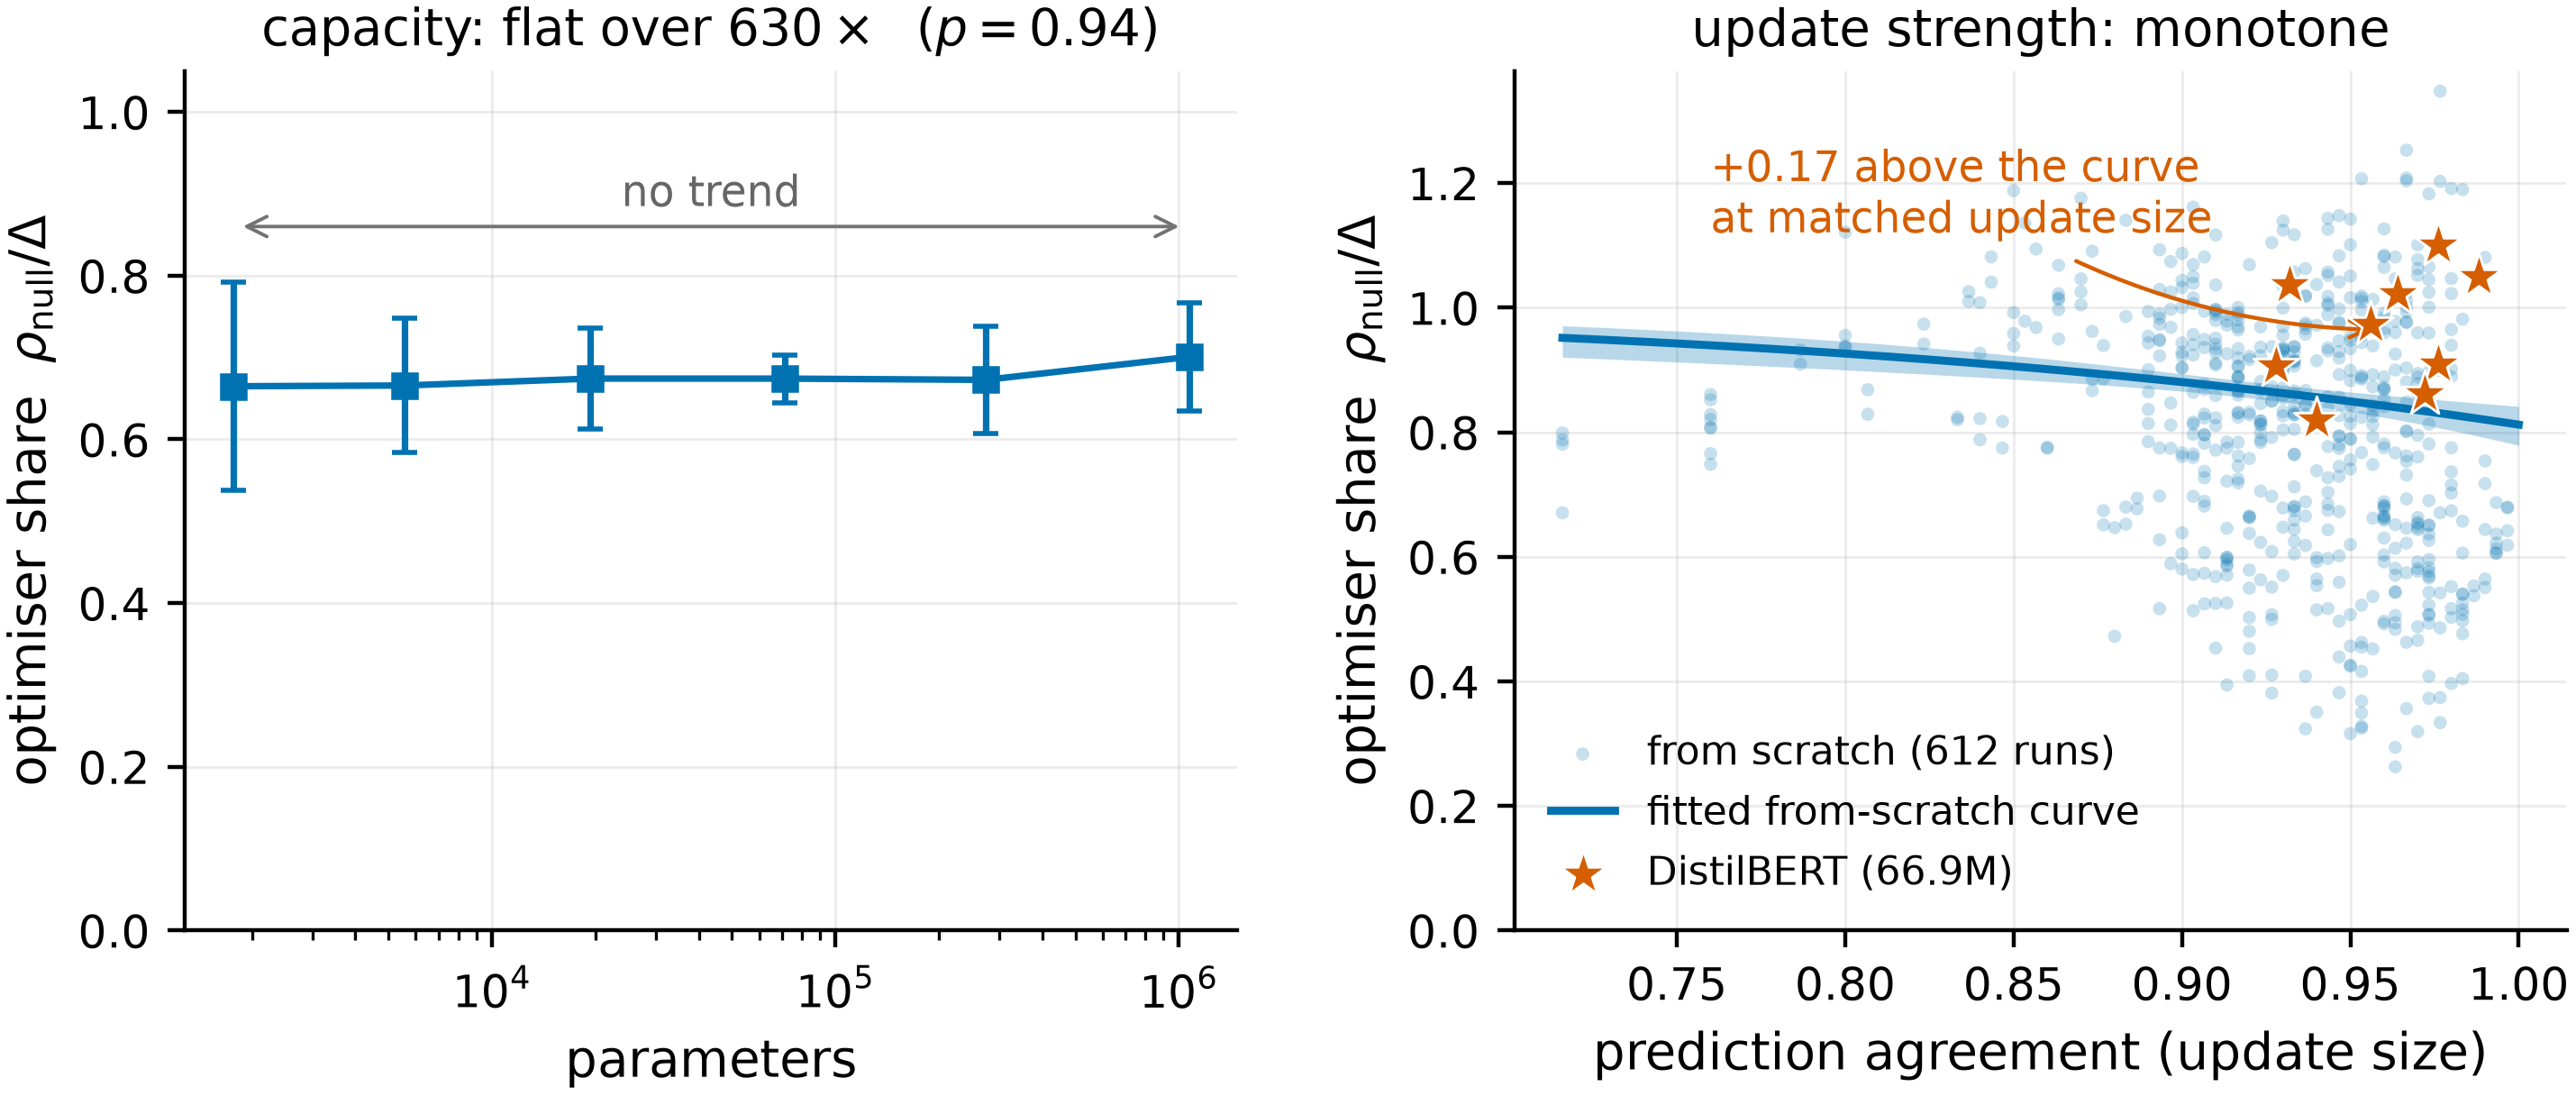
\includegraphics[width=\textwidth]{fig14_share_model.png}
\caption{What predicts the share of movement the optimiser reproduces, $\rnull/\Delta$. Left:
capacity does not predict it, with a logit-scale slope of $-0.007$ $[-0.197,+0.184]$, $p=0.94$,
across a 630$\times$ parameter range. Right: update strength does, monotonically; the fitted
from-scratch curve is shown with its 95\% interval, and DistilBERT sits $+0.173$ $[+0.104,+0.243]$
above it at matched update size.}
\label{fig:share}
\end{figure}

The share is $\rnull/\Delta$: the fraction of measured attribution change that the matched null
reproduces. A range on its own is a documented correlation; a model of it is a mechanism. Two
covariates are comparable across model classes. Prediction agreement measures how far an update moved
a model, and capacity measures its size. The width sweep holds the update fixed and varies parameters
630$\times$; the regime sweep holds capacity fixed and varies update strength. The share is bounded,
so it is modelled on a logit scale; a linear fit on the raw share extrapolates to impossible negative
values.

\section{Figure accessibility}
\label{app:figures}

Figures use the Okabe--Ito palette \citep{okabe2008} and encode every distinction redundantly, in
hatch for bars and in marker shape for lines, so that they survive monochrome printing and the
common colour-vision deficiencies. We simulated deuteranopia, protanopia and tritanopia by cone
collapse and checked pairwise separation for the colours that share each panel; where separation on
colour alone falls below threshold, the redundant encoding carries the distinction.

\end{document}
